% ============================================
% SPARROW AI - Complete Project Summary
% Addressing All Judging Criteria
% ============================================

\documentclass[11pt,a4paper]{article}

\usepackage[utf8]{inputenc}
\usepackage[T1]{fontenc}
\usepackage{lmodern}
\usepackage[margin=1in]{geometry}
\usepackage{graphicx}
\usepackage{booktabs}
\usepackage{array}
\usepackage{xcolor}
\usepackage{hyperref}
\usepackage{tikz}
\usepackage{enumitem}
\usepackage{fancyhdr}

% Colors
\definecolor{sparrowblue}{RGB}{37, 99, 235}
\definecolor{sparrowgreen}{RGB}{34, 197, 94}
\definecolor{sparrowred}{RGB}{239, 68, 68}
\definecolor{sparroworange}{RGB}{249, 115, 22}

% Header/Footer
\pagestyle{fancy}
\fancyhf{}
\fancyhead[L]{\textcolor{sparrowblue}{\textbf{Sparrow AI}}}
\fancyhead[R]{\textcolor{gray}{Project Summary}}
\fancyfoot[C]{\thepage}

\hypersetup{
    colorlinks=true,
    linkcolor=sparrowblue,
    urlcolor=sparrowblue
}

\begin{document}

% -------------------- Title --------------------
\begin{center}
{\Huge\textbf{\textcolor{sparrowblue}{SPARROW AI}}}\\[0.3cm]
{\LARGE ``Never Wing a Call Again''}\\[0.5cm]
{\Large Complete Project Summary}\\[0.3cm]
{\large AI Partner Catalyst Hackathon - ElevenLabs Challenge}\\[0.5cm]
\rule{14cm}{1pt}
\end{center}

\vspace{0.3cm}

\begin{center}
\begin{tabular}{ll}
\textbf{Live Demo:} & \url{https://sprrw.app}\\
\textbf{Repository:} & \url{https://github.com/hausorlabs/sparrow-ai}\\
\textbf{License:} & MIT (Open Source)\\
\end{tabular}
\end{center}

\vspace{0.5cm}

% -------------------- What is Sparrow --------------------
\section{What is Sparrow AI?}

Sparrow AI is a \textbf{voice-first sales training platform} that lets users practice cold calls, discovery conversations, and objection handling with realistic AI prospects powered by \textbf{ElevenLabs Conversational AI} and \textbf{Google Gemini}.

\begin{center}
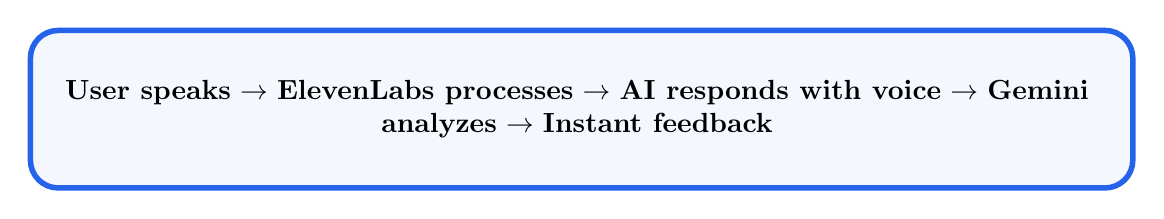
\begin{tikzpicture}
\node[draw=sparrowblue, line width=2pt, rounded corners=10pt, fill=sparrowblue!5, minimum width=14cm, minimum height=2cm, align=center] {
\begin{minipage}{13cm}
\centering
\textbf{User speaks} $\rightarrow$ \textbf{ElevenLabs processes} $\rightarrow$ \textbf{AI responds with voice} $\rightarrow$ \textbf{Gemini analyzes} $\rightarrow$ \textbf{Instant feedback}
\end{minipage}
};
\end{tikzpicture}
\end{center}

% -------------------- Problem --------------------
\section{The Problem}

\begin{center}

\begin{tikzpicture}
\node[draw=sparrowred, line width=2pt, rounded corners=8pt, fill=sparrowred!10, minimum width=12cm, minimum height=1cm] {
{\large\textbf{91\% of sales teams missed quota in 2024}}
};
\end{tikzpicture}
\end{center}

\begin{itemize}[leftmargin=*]
\item \textbf{3-6 months} average ramp time for new sales reps
\item \textbf{\$97,690} cost to replace one failed sales rep
\item \textbf{67\%} of reps miss their individual quota
\item \textbf{No safe place to practice} — reps learn on real prospects
\end{itemize}

Sales is a performance skill. You get better by \textit{doing}, not reading. But every practice opportunity today costs real money.

% -------------------- Solution --------------------
\section{Our Solution}

\subsection{Three Practice Modes}

\begin{table}[h]
\centering
\begin{tabular}{lll}
\toprule
\textbf{Mode} & \textbf{Goal} & \textbf{Skills Practiced}\\
\midrule
Cold Call Simulator & Book a meeting & Openers, attention, value props\\
Discovery Call & Uncover pain & Questions, listening, qualification\\
Objection Gauntlet & Handle pushback & Reframing, persistence, closing\\
\bottomrule
\end{tabular}
\end{table}

\subsection{Key Features}

\begin{enumerate}[leftmargin=*]
\item \textbf{AI Prospect Generation}: Gemini creates unique, realistic buyers with backstories
\item \textbf{Voice Conversations}: ElevenLabs enables natural speech interaction
\item \textbf{Real-time Scoring}: Instant feedback during and after calls
\item \textbf{Detailed Coaching}: Timestamped moments with specific suggestions
\item \textbf{Progress Tracking}: Skill development visualization over time
\end{enumerate}

% -------------------- Technology --------------------
\section{Technological Implementation}

\subsection{Core Integration}

\begin{table}[h]
\centering
\begin{tabular}{p{3.5cm}p{4cm}p{5.5cm}}
\toprule
\textbf{Technology} & \textbf{Provider} & \textbf{Use Case}\\
\midrule
Conversational AI & ElevenLabs & Real-time voice conversations\\
LLM Intelligence & Google Gemini 2.0 & Persona generation, call analysis\\
Fast Inference & Groq (Llama 3.1) & Real-time scoring\\
Database & Supabase & Data persistence\\
Authentication & Clerk & User management\\
Hosting & Vercel & Edge deployment\\
\bottomrule
\end{tabular}
\end{table}

\subsection{ElevenLabs Features Used}

\begin{itemize}[leftmargin=*]
\item \textbf{Conversational AI Agents}: Core voice interaction engine
\item \textbf{Dynamic Variables}: 15+ variables per session for persona customization
\item \textbf{Voice Library}: Multiple voices for different prospect personalities
\item \textbf{React SDK}: Seamless frontend integration (\texttt{@elevenlabs/react})
\item \textbf{Client Overrides}: Gender-appropriate voice selection
\end{itemize}

\subsection{Google Cloud / Gemini Usage}

\begin{itemize}[leftmargin=*]
\item \textbf{Model}: \texttt{gemini-2.0-flash-exp}
\item \textbf{Persona Generation}: Creates detailed prospect profiles from parameters
\item \textbf{Call Analysis}: Deep analysis of transcripts with structured JSON output
\item \textbf{Coaching}: Generates actionable feedback with specific suggestions
\end{itemize}

\subsection{Code Quality}

\begin{itemize}[leftmargin=*]
\item 100\% TypeScript for type safety
\item Next.js 15 with App Router
\item Modular component architecture
\item RESTful API design with proper error handling
\item Environment-based configuration
\end{itemize}

% -------------------- Design --------------------
\section{Design \& User Experience}

\subsection{User Journey}

\begin{enumerate}[leftmargin=*]
\item \textbf{Sign Up}: Quick authentication via Clerk
\item \textbf{Dashboard}: View stats, recent calls, improvement areas
\item \textbf{Select Mode}: Choose Cold Call, Discovery, or Objection Gauntlet
\item \textbf{Configure}: Pick industry, role, personality, difficulty
\item \textbf{Briefing}: Review AI-generated prospect details
\item \textbf{Call}: Natural voice conversation with real-time transcript
\item \textbf{Debrief}: Score card, key moments, full transcript
\item \textbf{Progress}: Track improvement over time
\end{enumerate}

\subsection{Design Principles}

\begin{itemize}[leftmargin=*]
\item \textbf{Voice-first}: Designed around natural conversation
\item \textbf{Clean UI}: Minimal distractions during calls
\item \textbf{Instant feedback}: No waiting for analysis
\item \textbf{Mobile-friendly}: Practice from anywhere
\end{itemize}

% -------------------- Impact --------------------
\section{Potential Impact}

\subsection{Market Opportunity}

\begin{table}[h]
\centering
\begin{tabular}{llp{6cm}}
\toprule
\textbf{Metric} & \textbf{Value} & \textbf{Calculation}\\
\midrule
TAM & \$5.7B & 5.7M B2B salespeople $\times$ \$1,000/year\\
SAM & \$1.5B & 2.6M inside sales reps $\times$ \$600/year\\
SOM & \$45M & 75K users at 10\% penetration (Year 5)\\
\bottomrule
\end{tabular}
\end{table}

\subsection{Who Benefits}

\begin{itemize}[leftmargin=*]
\item \textbf{SDRs}: 800,000+ in US need cold calling practice
\item \textbf{Inside AEs}: 1.2M+ need discovery and objection skills
\item \textbf{Sales Teams}: Reduce ramp time, lower turnover
\item \textbf{Career Changers}: Access quality training without expensive coaches
\end{itemize}

\subsection{Quantified Impact (at 75K users)}

\begin{itemize}[leftmargin=*]
\item 750,000+ practice calls per month
\item \$75M+ saved in reduced turnover costs
\item 15,000+ reps reaching quota who otherwise wouldn't
\end{itemize}

% -------------------- Creativity --------------------
\section{Quality of the Idea}

\subsection{What Makes Sparrow Unique}

\begin{enumerate}[leftmargin=*]
\item \textbf{Voice-first}: Not a chatbot — real voice conversations
\item \textbf{Dynamic personas}: Every practice session is unique
\item \textbf{Objective scoring}: AI removes manager bias
\item \textbf{Adaptive difficulty}: Adjusts to user skill level
\item \textbf{Instant availability}: Practice 24/7, unlimited sessions
\end{enumerate}

\subsection{Why Now}

\begin{itemize}[leftmargin=*]
\item \textbf{Voice AI maturity}: ElevenLabs reached human-quality in 2024
\item \textbf{LLM capabilities}: Gemini can roleplay convincingly
\item \textbf{Real-time inference}: Groq enables instant feedback
\item \textbf{Market pain}: 91\% quota miss rate demands new solutions
\end{itemize}

% -------------------- Learnings --------------------
\section{Findings \& Learnings}

\subsection{Technical Learnings}

\begin{enumerate}[leftmargin=*]
\item \textbf{ElevenLabs Dynamic Variables} are powerful for persona injection
\item \textbf{Voice override} requires enabling in Security settings
\item \textbf{Signed URLs} provide secure, temporary session access
\item \textbf{Gemini structured output} ensures consistent JSON responses
\item \textbf{Groq's speed} enables real-time scoring without latency
\end{enumerate}

\subsection{Product Learnings}

\begin{enumerate}[leftmargin=*]
\item Sales reps want \textit{realistic} pushback, not easy wins
\item Timestamped feedback is more valuable than overall scores
\item Voice quality directly impacts immersion and learning
\item Pre-call briefing increases engagement and roleplay commitment
\end{enumerate}

% -------------------- Conclusion --------------------
\section{Conclusion}

Sparrow AI demonstrates the power of combining ElevenLabs Conversational AI with Google Gemini to create a transformative voice-first application. The project:

\begin{itemize}[leftmargin=*]
\item[\checkmark] Deeply integrates both partner technologies
\item[\checkmark] Solves a real, quantifiable market problem
\item[\checkmark] Shows quality software development practices
\item[\checkmark] Delivers thoughtful user experience design
\item[\checkmark] Has significant potential impact on millions of sales professionals
\end{itemize}

\vspace{0.5cm}

\begin{center}

\begin{tikzpicture}
\node[draw=sparrowblue, line width=2pt, rounded corners=10pt, fill=sparrowblue, minimum width=8cm, minimum height=1cm, align=center] {
{\large\textcolor{white}{\textbf{sprrw.app}}}
};
\end{tikzpicture}
\end{center}

\vspace{0.5cm}

\begin{center}
\textit{``Never wing a call again.''}
\end{center}

\end{document}
